% Chapter 1
\chapter{Definición del problema u oportunidad} % Main chapter title
\label{sec:problema} % For referencing the chapter elsewhere, use

Este capítulo debe contener la exposición general del problema. Con respecto al problema se debe responder las siguientes preguntas:
\begin{itemize}
	\item	¿Cuál es el problema u oportunidad abordado por el proyecto? ¿Es posible cuantificarlo?
	\item	¿Cuáles son las causas de la existencia de este problema u oportunidad? Haga referencia a publicaciones y/u otros antecedentes que validen estas causas.
	\item Explique cómo la memoria ayudará a abordar este problema.
	
\end{itemize}

\section{Ejemplos de latex}

Sed ullamcorper quam eu nisl interdum at interdum enim egestas. Aliquam placerat justo sed lectus lobortis ut porta nisl porttitor. Vestibulum mi dolor, lacinia molestie gravida at, tempus vitae ligula. Donec eget quam sapien, in viverra eros. Donec pellentesque justo a massa fringilla non vestibulum metus vestibulum. Vestibulum in orci quis felis tempor lacinia. Vivamus ornare ultrices facilisis. Ut hendrerit volutpat vulputate. Morbi condimentum venenatis augue, id porta ipsum vulputate in. Curabitur luctus tempus justo. Vestibulum risus lectus, adipiscing nec condimentum quis, condimentum nec nisl. Aliquam dictum sagittis velit sed iaculis. Morbi tristique augue sit amet nulla pulvinar id facilisis ligula mollis. Nam elit libero, tincidunt ut aliquam at, molestie in quam. Aenean rhoncus vehicula hendrerit.

\begin{figure}[th]
	\centering
	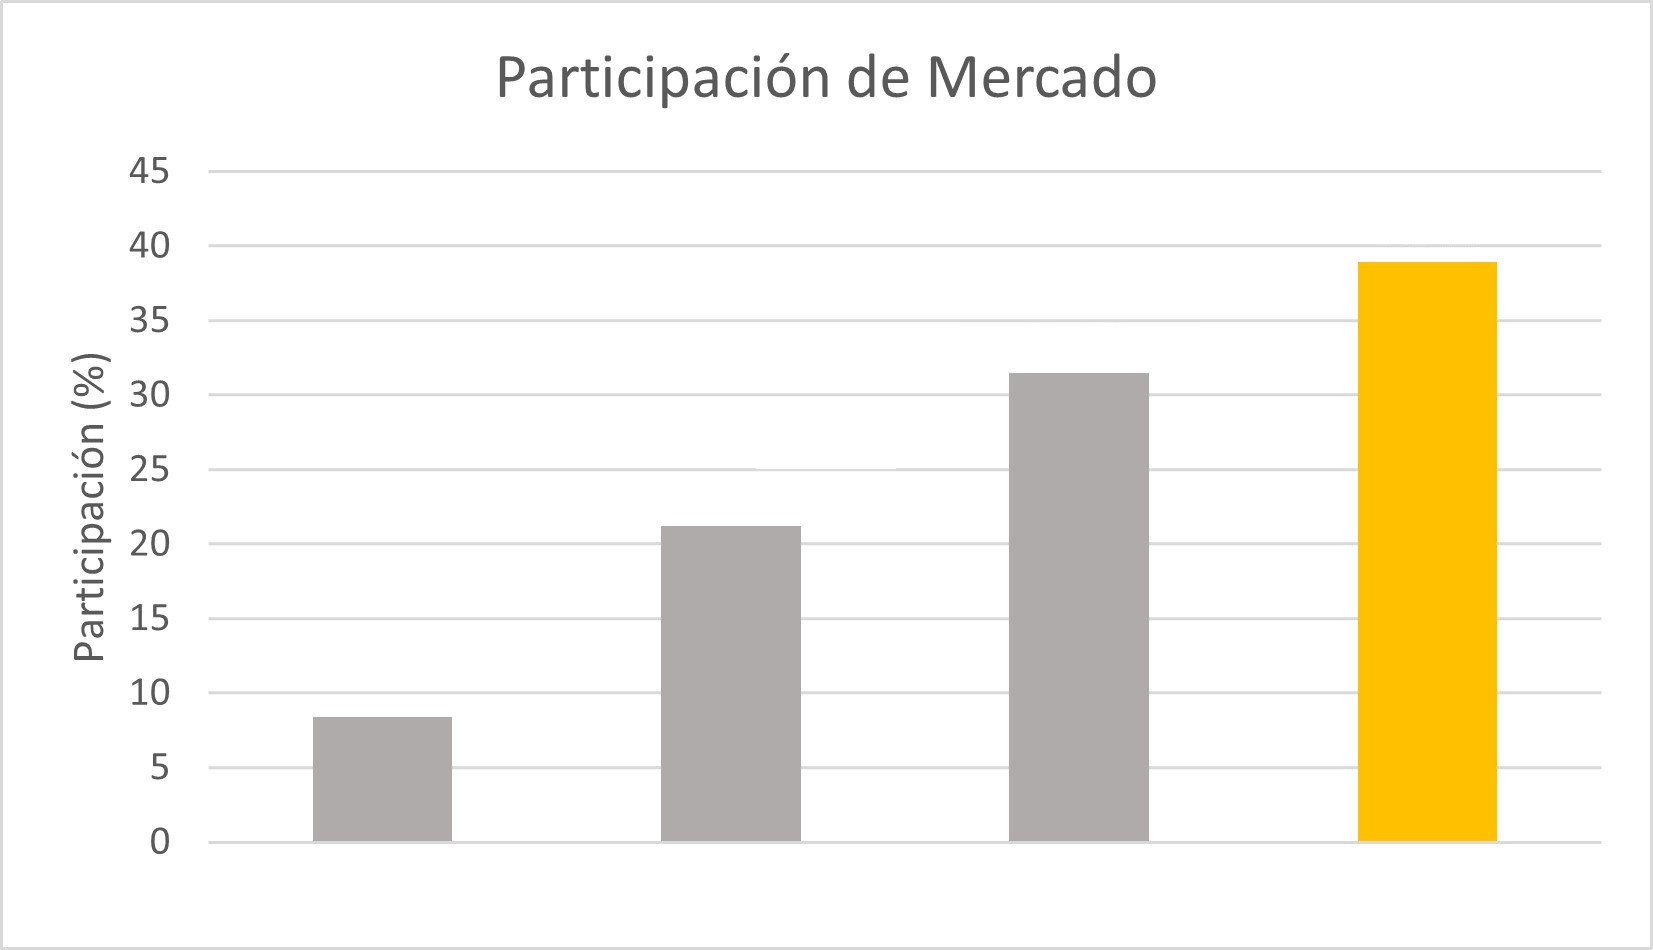
\includegraphics[width=10cm]{Figures/Ejemplo}
	\caption{Comparación de la participación de mercado entre mutuales, a enero 2020.}
	\label{fig:Ejemplo}
\end{figure}

% Citando Figura~\ref{fig:Ejemplo} de la sección~\ref{sec:problema}

Lista de items
\begin{itemize}
	\item \textbf{Componente A:} Sed ullamcorper quam eu nisl interdum at interdum enim egestas. Aliquam placerat justo sed lectus lobortis ut porta nisl porttitor. Vestibulum mi dolor, lacinia molestie gravida at, tempus vitae ligula. Donec eget quam sapien, in viverra eros. Donec pellentesque justo a massa fringilla non vestibulum metus vestibulum. Vestibulum in orci quis felis tempor lacinia. Vivamus ornare ultrices facilisis. Ut hendrerit volutpat vulputate. Morbi condimentum venenatis augue, id porta ipsum vulputate in.
	\item \textbf{Componente B:} Sed ullamcorper quam eu nisl interdum at interdum enim egestas. Aliquam placerat justo sed lectus lobortis ut porta nisl porttitor. Vestibulum mi dolor, lacinia molestie gravida at, tempus vitae ligula. Donec eget quam sapien, in viverra eros. Donec pellentesque justo a massa fringilla non vestibulum metus vestibulum. Vestibulum in orci quis felis tempor lacinia. Vivamus ornare ultrices facilisis. Ut hendrerit volutpat vulputate. Morbi condimentum venenatis augue, id porta ipsum vulputate in.
\end{itemize}

Lista enumerada
\begin{enumerate}
	\item \textbf{Componente A:} Sed ullamcorper quam eu nisl interdum at interdum enim egestas. Aliquam placerat justo sed lectus lobortis ut porta nisl porttitor. Vestibulum mi dolor, lacinia molestie gravida at, tempus vitae ligula. Donec eget quam sapien, in viverra eros. Donec pellentesque justo a massa fringilla non vestibulum metus vestibulum. Vestibulum in orci quis felis tempor lacinia. Vivamus ornare ultrices facilisis. Ut hendrerit volutpat vulputate. Morbi condimentum venenatis augue, id porta ipsum vulputate in.
	\item \textbf{Componente B:} Sed ullamcorper quam eu nisl interdum at interdum enim egestas. Aliquam placerat justo sed lectus lobortis ut porta nisl porttitor. Vestibulum mi dolor, lacinia molestie gravida at, tempus vitae ligula. Donec eget quam sapien, in viverra eros. Donec pellentesque justo a massa fringilla non vestibulum metus vestibulum. Vestibulum in orci quis felis tempor lacinia. Vivamus ornare ultrices facilisis. Ut hendrerit volutpat vulputate. Morbi condimentum venenatis augue, id porta ipsum vulputate in.
\end{enumerate}

% Citas a libro \cite{ejemploLibro} o paper~\cite{ejemploPaper}. Usted puede agregar otros tipos como journal o techincal report
